% =============================================================
% SECTION III: SYSTEM ARCHITECTURE
% =============================================================
\section{System Architecture}
\label{sec:architecture}

NyayaSahaya adopts a three-tier architecture comprising: (i)~a web-based presentation layer for end users, (ii)~a central orchestration layer that coordinates retrieval, analysis, and policy enforcement, and (iii)~a trusted edge component that anchors authentication. This separation preserves responsiveness at the interface while isolating sensitive operations from the client environment. Fig.~\ref{fig:system_arch} summarizes the system topology at an abstract level.

\begin{figure*}[!t]
\centering
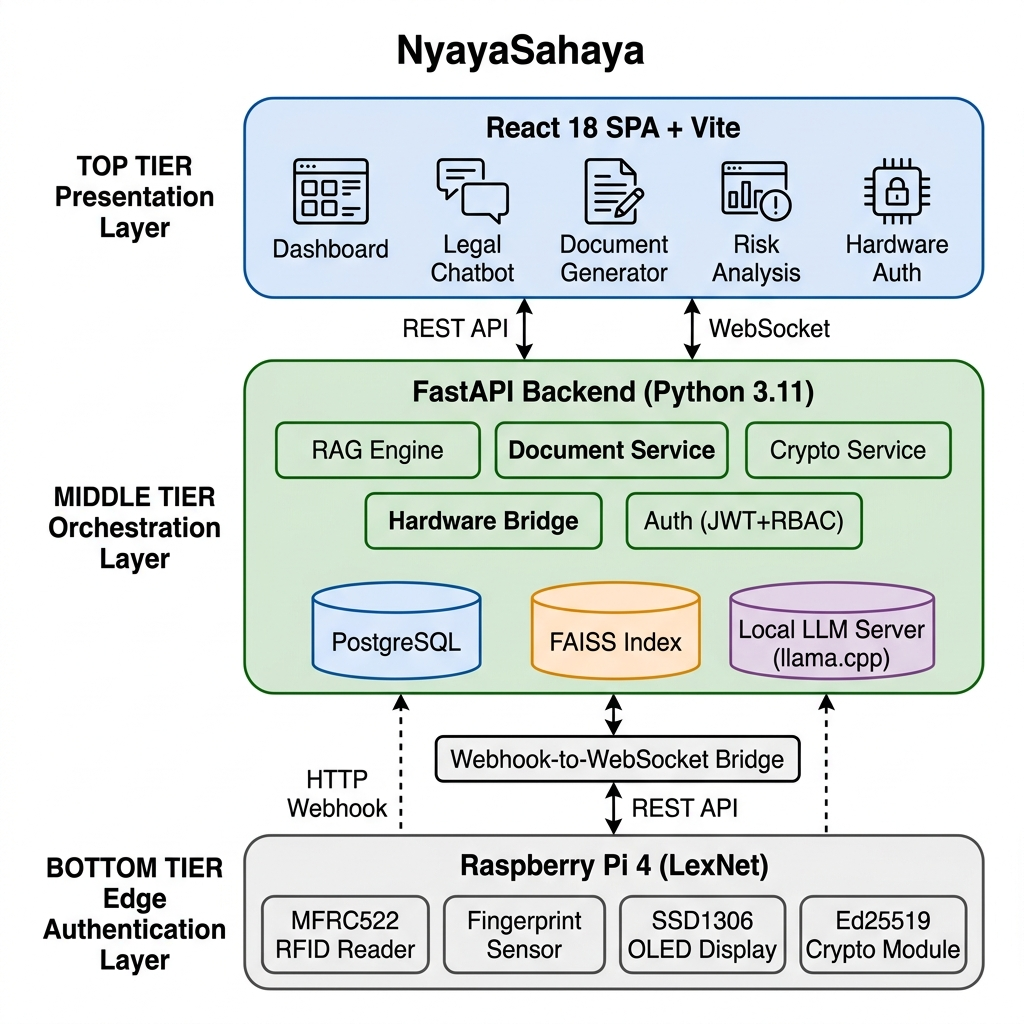
\includegraphics[width=0.70\textwidth]{figures/system_architecture.png}
\caption{Abstract system architecture of NyayaSahaya showing the presentation layer, orchestration layer, and trusted edge component, along with their high-level interactions.}
\label{fig:system_arch}
\end{figure*}

\subsection{Frontend Layer}

The presentation layer provides a guided interface for legal inquiry, document management, and verification monitoring. It emphasizes clarity, minimal steps, and consistent feedback to reduce cognitive load for non-expert users. Role-aware views present only the actions relevant to each user category while keeping sensitive controls behind appropriate permissions. The interface also surfaces explanations and next-step prompts to make complex workflows feel linear and understandable.

\subsection{Backend Orchestration Layer}

The orchestration layer coordinates retrieval, analysis, signing, and access control as cohesive services. It enforces policy boundaries, mediates requests between the interface and the trusted edge component, and maintains auditability across document workflows. The implementation is modular to support future extensions without exposing internal mechanics to the client. It also normalizes inputs and outputs to keep user-facing responses consistent even when internal processes vary.

\subsection{Edge Authentication Layer (LexNet)}

The edge authentication layer performs presence verification and emits signed assertions that can be audited by the orchestration layer. The device is treated as a trust anchor, and its responsibilities are deliberately scoped to authentication and integrity signaling. This separation prevents client-side tampering and keeps verification logic outside the presentation layer.

\subsection{Data Persistence Layer}

NyayaSahaya maintains a secure data store for users, documents, and analysis artifacts. A tamper-evident ledger records document provenance and integrity metadata, while access control policies govern sharing and visibility. This structure enables traceability of document actions without exposing sensitive internal representations.

\subsection{Communication Architecture}

Communication between tiers follows an event-driven pattern. The orchestration layer mediates edge authentication signals and exposes only sanitized status updates to the interface, ensuring that the client never communicates directly with the trusted device. This separation preserves a clean security boundary and supports real-time feedback without exposing implementation details. The flow is designed to be robust to intermittent connectivity while preserving a clear audit trail.
